%%
%% This is file `sample-sigconf.tex',
%% generated with the docstrip utility.
%%
%% The original source files were:
%%
%% samples.dtx  (with options: `sigconf')
%% 
%% IMPORTANT NOTICE:
%% 
%% For the copyright see the source file.
%% 
%% Any modified versions of this file must be renamed
%% with new filenames distinct from sample-sigconf.tex.
%% 
%% For distribution of the original source see the terms
%% for copying and modification in the file samples.dtx.
%% 
%% This generated file may be distributed as long as the
%% original source files, as listed above, are part of the
%% same distribution. (The sources need not necessarily be
%% in the same archive or directory.)
%%
%% The first command in your LaTeX source must be the \documentclass command.
\documentclass[sigconf]{acmart}

%% Remove copyroght notes for lecture/preprint purposes
\settopmatter{printacmref=false}
\setcopyright{none}
\renewcommand\footnotetextcopyrightpermission[1]{}
\pagestyle{plain}

\setcopyright{none}
\makeatletter
\renewcommand\@formatdoi[1]{\ignorespaces}
\makeatother

\acmConference{}{}{}

%%
%% \BibTeX command to typeset BibTeX logo in the docs
\AtBeginDocument{%
  \providecommand\BibTeX{{%
    \normalfont B\kern-0.5em{\scshape i\kern-0.25em b}\kern-0.8em\TeX}}}

%% Rights management information.  This information is sent to you
%% when you complete the rights form.  These commands have SAMPLE
%% values in them; it is your responsibility as an author to replace
%% the commands and values with those provided to you when you
%% complete the rights form.
%\setcopyright{acmcopyright}
%\copyrightyear{2018}
%\acmYear{2018}
%\acmDOI{10.1145/1122445.1122456}

%% These commands are for a PROCEEDINGS abstract or paper.
%\acmConference[Woodstock '18]{Woodstock '18: ACM Symposium on Neural
%  Gaze Detection}{June 03--05, 2018}{Woodstock, NY}
%\acmBooktitle{Woodstock '18: ACM Symposium on Neural Gaze Detection,
%  June 03--05, 2018, Woodstock, NY}
%\acmPrice{15.00}
%\acmISBN{978-1-4503-XXXX-X/18/06}


%%
%% Submission ID.
%% Use this when submitting an article to a sponsored event. You'll
%% receive a unique submission ID from the organizers
%% of the event, and this ID should be used as the parameter to this command.
%%\acmSubmissionID{123-A56-BU3}

%%
%% The majority of ACM publications use numbered citations and
%% references.  The command \citestyle{authoryear} switches to the
%% "author year" style.
%%
%% If you are preparing content for an event
%% sponsored by ACM SIGGRAPH, you must use the "author year" style of
%% citations and references.
%% Uncommenting
%% the next command will enable that style.
%%\citestyle{acmauthoryear}

 
%%
%% end of the preamble, start of the body of the document source.
\begin{document}

%%
%% The "title" command has an optional parameter,
%% allowing the author to define a "short title" to be used in page headers.
\title{Sicherheit und Privatheit von Push-Notification-Services für mobile Apps}

%%
%% The "author" command and its associated commands are used to define
%% the authors and their affiliations.
%% Of note is the shared affiliation of the first two authors, and the
%% "authornote" and "authornotemark" commands
%% used to denote shared contribution to the research.
\author{Chantal Bruns}
\affiliation{%
  \institution{Hochschule Bonn-Rhein-Sieg}
}
\email{chantal.bruns@smail.inf.h-brs.de}

\author{Issam Hbib}
\affiliation{%
  \institution{Hochschule Bonn-Rhein-Sieg}
}
\email{issam.hbib@smail.inf.h-brs.de}

\author{Robert Bargon}
\affiliation{%
  \institution{Hochschule Bonn-Rhein-Sieg}
}
\email{robert.bargon@smail.inf.h-brs.de}

%%
%% By default, the full list of authors will be used in the page
%% headers. Often, this list is too long, and will overlap
%% other information printed in the page headers. This command allows
%% the author to define a more concise list
%% of authors' names for this purpose.
\renewcommand{\shortauthors}{Bruns, Hbib, Bargon}

%%
%% The abstract is a short summary of the work to be presented in the
%% article.
\begin{abstract}
  In dieser wissenschaftlichen Arbeit wurde untersucht, wie oft Push Notification von App Entwicklern benutzt wird.
  Dabei kam heraus, dass sichere Push Notification im medizinischen Bereich am meisten benutzt wurden, aber
  die Anzahl im Vergleich zur Gesamtanzahl überprüfter Apps dennoch ernüchternd ist.
\end{abstract}

%%
%% The code below is generated by the tool at http://dl.acm.org/ccs.cfm.
%% Please copy and paste the code instead of the example below.
%%
\begin{CCSXML}
<ccs2012>
  <concept>
  <concept_id>10002978.10003022.10003028</concept_id>
  <concept_desc>Security and privacy~Domain-specific security and privacy architectures</concept_desc>
  <concept_significance>300</concept_significance>
  </concept>
</ccs2012>
\end{CCSXML}

\ccsdesc[500]{Security and privacy~Domain-specific security and privacy architectures}

%%
%% Keywords. The author(s) should pick words that accurately describe
%% the work being presented. Separate the keywords with commas.
\keywords{push notifications, encryption, cloud messaging services}

%%
%% This command processes the author and affiliation and title
%% information and builds the first part of the formatted document.
\maketitle

\section{Introduction}

Push Notification ist ein unerlässlicher Teil der heutigen Apps. 
Sei es Nutzer*innen über neue Nachrichten einer Chat-App 
zu benachrichtigen oder auf eine überfällige Periode hinzuweisen, 
Ihre Benutzung ist vielfältig und birgt damit auch Risiken, da sie 
private Daten beinhalten können.

Im Folgenden wird untersucht, ob von den Entwicklern
sichergestellt wird, dass der Inhalt der
Push Notifications nicht von unberechtigten Entitäten mitgelesen 
werden kann.

\section{Grundlagen von Push-Benachrichtigungen}

\subsection{Was ist Firebase?}

Firebase ist eine Entwicklungsplattform, mit welcher es möglich ist 
Apps (mobil und webbasiert) in der Google Cloud Plattform zu entwickeln.
Es bietet durch verschiedene Services, den Entwicklern die Möglichkeit, 
die App-Entwicklung zu beschleunigen und die Stabilität und Leistung 
zu überwachen. Darunter auch die Push-Notifications, welche im Folgenden 
genauer erläutert werden \cite{cloudwuerdig}.

\subsection{Typischer Push-Notification-Flow}

\begin{figure}[H]
  \centering
  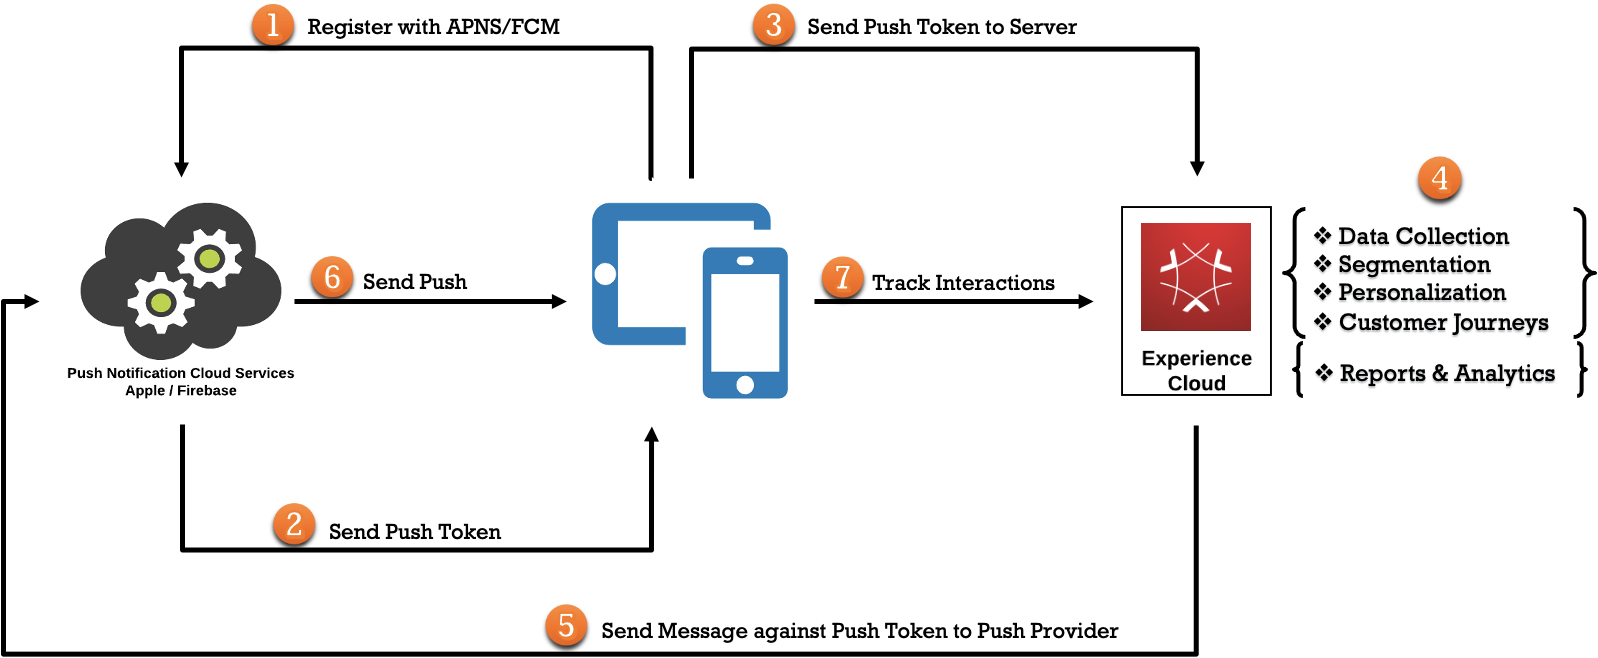
\includegraphics[width=\linewidth]{sample-flow}
  \caption{Push Notification Flow von Anshika Agarwal (\url{https://medium.com/adobetech/securing-push-notifications-in-mobile-apps-a23b6c20139e}).}
  \Description{Flussdiagramm eines typischen Push Notification Flows}
\end{figure}

Um die Funktionalität der Push-Benachrichtigungen herzustellen, 
werden die SDK-APIs der mobilen Plattform z.B. Apple iOS oder Android, 
verwendet, um sich damit bei einem Cloud-Messaging-Anbieter 
registrieren zu können. Dazu gehören Apple Push Notification Service 
(APNs) für iOS und Firebase Cloud Messaging (FCM) für Android.
Zuerst sendet der Cloud-Messaging-Anbieter ein Push-Token, welches wie 
eine Adresse funktioniert, mit dem es möglich ist das Gerät und die 
mobile App als Empfänger der Nachricht zu identifizieren.
Daraufhin wird das Push-Token von der mobilen App an den Server einer 
Customer-Engagement-Plattform gesendet, denn das Push-Token muss dem 
Server bekannt sein, um eine Push-Benachrichtigung an den Empfänger 
senden zu können.
Die Sicherheit, dass die personalisierten Inhalte nur vom 
beabsichtigten Benutzer empfangen werden, ist durch die Eins-zu-Eins 
Zuordnung zwischen dem Push-Token und der Kennung des Benutzers vom 
System gewährleistet.
Der Remote-Server sammelt die Nutzerdaten und Interaktionen und gibt 
den App-Entwicklern die Möglichkeit z.B. den Nachrichteninhalt so zu 
personalisieren, dass er auf die Nutzungsmuster und -attribute der 
Kunden angepasst ist.
Die personalisierte Nachricht wird an das Push-Token gebunden und 
vom Remote-Server an den Cloud-Messaging-Dienst der mobilen 
Plattform gesendet.
Der Nachrichteninhalt wird dann vom Cloud-Messaging-Dienst an das 
richtige Gerät und die mobile App gesendet und dann anschließend als 
Benachrichtigung angezeigt \cite{agarwal}.

\subsection{Firebase Cloud Messaging für Android}

Um FCM-basierte Push-Benachrichtigungen in einer 
Android-App zu implementieren, werden eine mobile App, eine Verbindung 
zum FCM-Server und ein Push-Server eines Drittanbieters benötigt.
Zuerst muss Firebase zu dem Android-App-Projekt hinzugefügt werden. 
Danach ist es erforderlich sich bei FCM zu registrieren, um das 
FCM-Registrierungstoken zu erhalten. Um dann anschließend eine 
Verbindung mit den FCM-Servern herzustellen, muss das FCM-Token 
in der Android-App konfiguriert werden. Nun wird ein Push-Server 
eines Drittanbieters benötigt, damit Benachrichtigungen von der 
mobilen App an den FCM-Server gesendet werden können.
Hierfür wird oftmals der Google Play Store verwendet, der die 
Einrichtung mit den Google Play-Diensten APK erfordert. Es können 
aber auch Push-Benachrichtigungsserver eines Drittanbieters verwendet 
werden \cite{firebase}.

\subsection{Push-Notifications für Apple}

Für iOS funktionieren Push-Notifications ähnlich wie bei Android 
mit dem Unterschied, dass die App mit dem Apple Push Notification 
Service kommuniziert. Hierfür wird ein Apple Push Notification 
Authentication Key für den Apple Developer Account benötigt. 
Zuerst fordert iOS ein Gerätetoken vom Apple Push Notification 
Service (APNs) an. Danach empfängt die iOS-App das Token, mit 
welchem Push-Benachrichtigungen an die identifizierte Anwendung 
gesendet werden. Zum Schluss sendet der Server einer 
Customer-Engagement-Plattform, die Benachrichtigung an den APNs 
und dann identifiziert der APNs das iOS-Gerät und die iOS-App, 
an die die Benachrichtigung gesendet werden soll \cite{apple}.

\section{Sichere Push-Notifications}

\subsection{Grundlagen von sicheren Push Notifications}

Wenn eine Benachrichtigung eines App-Anbieters über einen Messaging 
Dienst wie FCM zum Endgerät gelangen soll, ist die Kommunikation 
zwischen Entwickler und Messaging Dienst, sowie die Kommunikation 
zwischen Messaging Dienst und Endgerät durch TLS verschlüsselt, 
jedoch wird der eigentliche Inhalt der Benachrichtigungen in Klartext 
übermittelt \cite{capillary}. So handelt es sich dabei nicht um eine 
Ende-zu-Ende Verschlüsselung zwischen App und Entwickler und der Inhalt der Nachricht kann von 
beispielsweise Google mitgelesen werden.
Google selbst empfiehlt die Nutzung von Bibliotheken von Drittanbietern, 
unter anderem das hauseigene Capillary \cite{firebase2}.

Apple hingegen bietet das UNNotificationServiceExtension Objekt an, 
womit verschlüsselte Push-Notifications von der App entschlüsselt 
werden können. Dabei muss der versendete Notification Payload den 
Json Key „mutable-content“ mit dem Wert 1 beinhalten, damit das 
UNNotificationServiceExtension Objekt die verschlüsselte Notification 
entschlüsselt, bevor dessen Inhalt im Gerät angezeigt wird \cite{apple1}\cite{apple2}.

Bedenklich ist die Tatsache, dass alle Benachrichtigung 
einer Person zugeordnet werden können und die Anbieter dieser Messaging 
Dienste meist US-amerikanische Firmen sind, welche beispielsweise 
Daten an Behörden weiterreichen müssten, falls gefordert \cite{google2}.

Um den Inhalt von Push-Benachrichtigungen vor den Messaging Diensten 
zu schützen, muss der App-Anbieter sich also selbst um eine 
Ende-zu-Ende-Verschlüsselung kümmern.

Dies kann besonders wichtig sein, wenn es sich um Benachrichtigungen 
handelt, welche sensible Personen Informationen enthalten. Wenn es 
sich um Benachrichtigungen von Instant Messaging Diensten handelt, 
oder sensiblere Daten von Banking Apps oder vergleichbarem, 
ist eine Verschlüsselung der Inhalte besonders erstrebenswert.

Eine solche Ende-zu-Ende-Verschlüsselung lässt sich über eine 
asymmetrische Verschlüsselung realisieren, wobei das 
Endgerät das Schlüsselpaar erzeugt und den öffentlichen Schlüssel an 
den Entwickler schickt und dabei den Messaging Dienst außen vor lässt. 
Dabei muss man nicht die Funktionsweise des Messaging Dienstes 
einschränken und kann vorhandene Technologien weiter nutzen.



\subsection{Beispiel eines sicheren Notification Flow}

\begin{figure}[H]
  \centering
  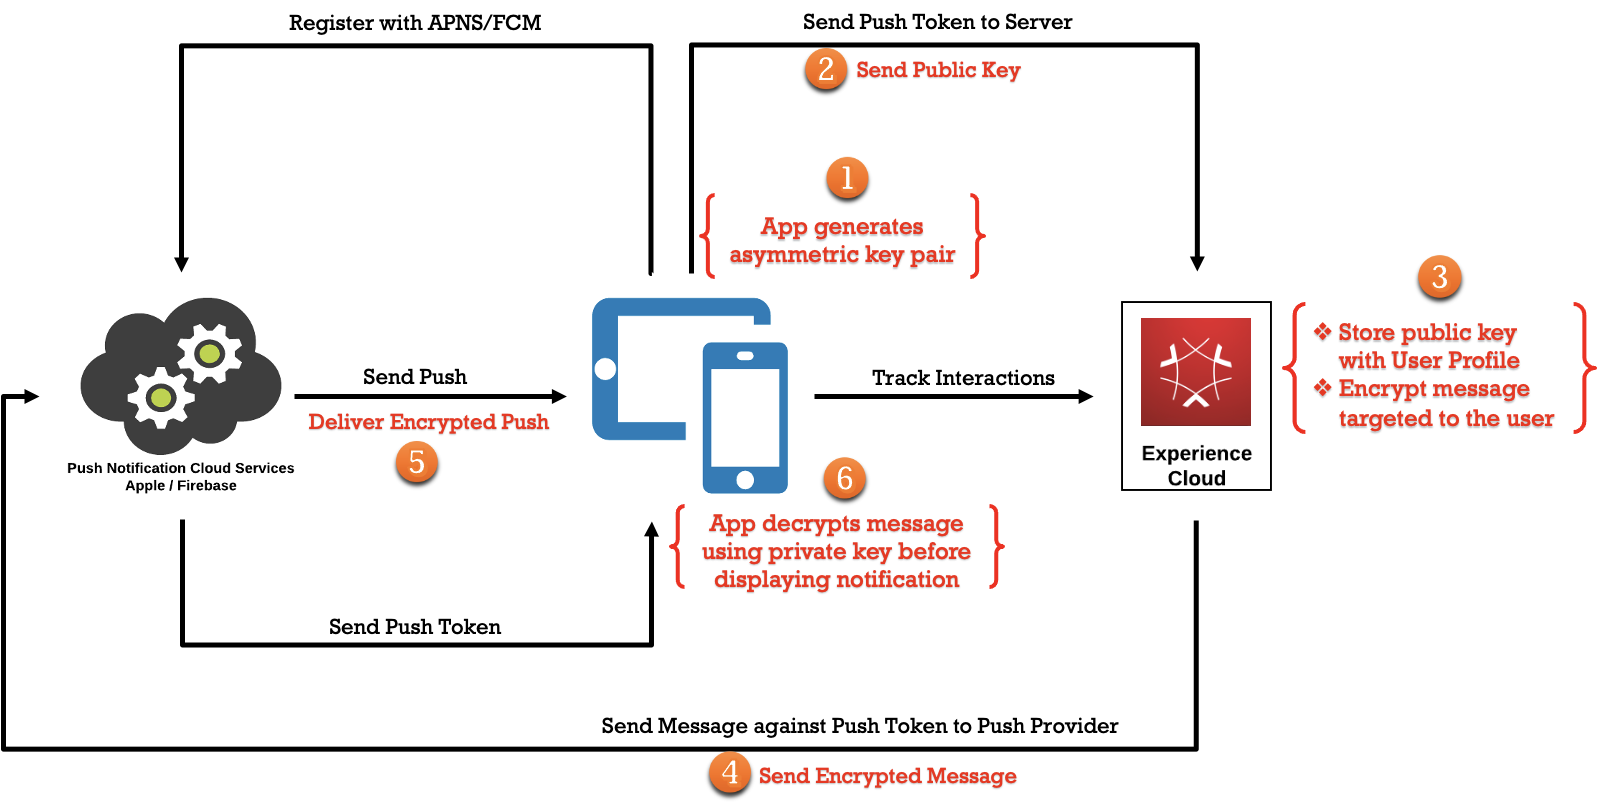
\includegraphics[width=\linewidth]{sample-secureflow}
  \caption{Sicherer Push Notification Flow von Anshika Agarwal (\url{https://medium.com/adobetech/securing-push-notifications-in-mobile-apps-a23b6c20139e}).}
  \Description{Flussdiagramm eines sicheren Push Notification Flows}
\end{figure}

Nachfolgend wird das Beispiel eines sicheren Notification Flow erläutert \cite{agarwal}.

1. Der Anwender erzeugt auf seinem Endgerät automatisiert ein 
Schlüsselpaar, bestehend aus einem öffentlichen und einem privaten 
Schlüssel.

2. Der öffentliche Schlüssel wird dem Entwickler nun über einen direkten 
Kommunikationsweg übermittelt.

3. Der Entwickler speichert nun diesen Schlüssel und verknüpft ihn Lokal 
mit dem Messaging Dienst Identifier für das spezifische Endgerät. 
Nun ist er in der Lage mit dem öffentlichen Schlüssel seine ausgehenden 
Benachrichtigungen zu verschlüsseln.

4. Die verschlüsselte Benachrichtigung wird nun dem Messaging Dienst 
übermittelt, welcher diese, für ihn unlesbare Nachricht, an das Endgerät 
übermittelt.

5. Das Endgerät kann bei Erhalt der Benachrichtigung, durch seinen lokal 
gespeicherten privaten Schlüssel den Inhalt entschlüsseln und die 
Benachrichtigung kann dem Nutzer angezeigt werden.

\subsection{Umsetzung in Open Source Projekten}

Capillary ist eine Bibliothek von Google, welche Drittanbieter, eine End-zu-End 
Verschlüsselung über Firebase Cloud Messaging ermöglicht \cite{capillary}. Unter anderem 
bietet sie die Schlüsselgeneration als auch Registrierung der erstellten 
asymmetrischen Schlüssel mit dem Developer Application Server, der die 
Benachrichtigungen verschlüsselt über Firebase an die App mit Capillary 
versendet. Zudem bietet Capillary die Entschlüsselung und Verschlüsselung 
der Notification clientseitig in der App als auch serverseitig an.

Capillary bietet noch weitere Funktionen, wie zum Beispiel, dass ein gestohlenes 
Endgerät die Möglichkeit der Entschlüsselung noch eingehender Benachrichtigungen 
entzogen werden kann.

Die Popularität dieser Bibliothek scheint, gemessen anhand der ungefähr 
450 Github Stars Stand Dezember 2021, eingeschränkt. Der letzte Commit 
war im Dezember 2018, womit das Projekt verlassen ausschaut.

Eine weitere Möglichkeit verschlüsselte Notifications zu senden, 
besteht über das Extensible Messaging and Presence Protocol (XMPP).
XMPP selbst ist ein Standard der Internet Engineering Task Force (IETF), 
welcher Technologien wie instant messaging, Push Notifications, voice und 
video calls über XML ermöglicht \cite{xmpp}\cite{xmpp3}.  Dieser Standard definiert zudem die 
End-zu-End Verschlüsselung als auch Signierung von versendeten Objekten. 
Dies kann verwendet werden, um Push Notifications zu verschlüsseln \cite{xmpp2}.

\section{Prototyp}

\subsection{Herausforderung}
Der erste Ansatz war die Push Notifications auf der Netzwerkebene zu analysieren,
aber durch die Tatsache, dass die Pakete TLS verschlüsselt sind, wie wir in unserer späteren
Recherche herausgefunden haben, kamen wir auf die Idee, uns die Apps direkt anzuschauen. Zunächst
war die Herausforderung, die aktuelle Version einer App aus einer sicheren Quelle herunterzuladen.
Dazu diente das Fork vom Python Projekt GooglePlayAPI von TheZ3ro \cite{googleplayapi}.
Danach ergab sich die Frage, wie man generell eine App in APK-Form analysieren kann.
Der für uns logische Schritt war demnach die App mit Jadx \cite{jadx} zu dekompilieren und darauf Stringabgleiche
durchzuführen. In den ersten Testläufen innerhalb einer virtuellen Machine wurden Performane-Einbußen festgestellt,
da Jadx für das Dekompilieren einer einzelnen App mehrere Minuten brauchen könnte, was bei einer Liste von vielen hunderten
Apps viele Stunden in Anspruch nehmen könnte, sodass sich die weitere Frage ergab, wie man den ganzen Prozess effizienter gestalten kann
und warum man überhaupt eine App dekompiliert. Als Antwort auf die zweite Frage stellten wir fest, dass das Dekompilieren
einer App dazu gedacht ist, den Code Flow dieser App in menschlich-lesbarer Form darzustellen, allerdings 
benötigt unser Analyse-Skript keinen menschlich-lesbaren Code, sondern führt Stringabgleiche mit statischen Werten durch,
die sich auch in der Rohform einer entpackten App finden lassen, wodurch der Prozess effizienter wird, da das 
Entpacken weniger Zeit in Anspruch nimmt als das Dekompilieren und somit die Antwort auf die erste Frage ist.

Zudem stellte sich die Frage was analysiert werden sollte. Dabei konnten wir herausfinden,
dass Google Play hochgeladene Apps in bestimmte Kategorien unterteilt, sodass sich für uns die Idee ergab,
eine bestimmte Anzahl an Apps je Kategorie zu analysieren und miteinander zu vergleichen. Wir haben uns für die Kategorien
„Health\_And\_Fitness“, „Medical“ und „Communication“ entschieden, da Apps in diesen Bereichen oft mit privaten Daten 
in Kontakt treten können. Danach stellte sich die Herausforderung wie man eine entsprechende Liste scrapen kann.
Hierbei wurde zunächst versucht dies über den Browser zu realisieren, aber die Google Play Seite im Browser zeigt nur eine geringe Anzahl Apps
pro Kategorie an. Daraufhin wurde versucht mittels Dekompilierung der Google Play App und Hooking mit Frida \cite{frida}
an die Daten zu gelangen, was sich als komplex erwies. Während der Recherche trafen wir auf die Seite "androidrank.org", welche
aktuelle Top 500 App Listen pro Kategorie anzeigt.

\subsection{Problematik der Analyse}
Eine Ende-zu-Ende Verschlüsselung kann von einem Entwickler unterschiedlich implementiert werden,
sodass eine automatische Überprüfung kompliziert wäre, da manche Apps zum Beispiel obfuskiert werden können.
Unsere Suche bezieht sich jedoch nur auf den Stringabgleich der Bibliotheksnamen, was die Analyse vereinfacht
und dennoch eine erste grobe Momentaufnahme liefert.

\subsection{Umsetzung}
Im Rahmen des Projektes sollte überprüft werden, wie oft unsichere Push 
Notifications in Apps benutzt wurden. Hierfür wurden nur Android Apps 
betrachtet. Zu den Analysekriterien gehört die Benutzung von 
"NotificationCompat" \cite{google} mithilfe von einem Stringabgleich, welche zu den 
Android Schnittstellen gehört und das Senden von Push Nachrichten ermöglicht, sowie auf "onMessageReceived" \cite{firebase3}, welche 
benutzt wird, um Push Notification von Firebase zu empfangen. 
Wenn diese vorhanden sind, wird davon ausgegangen, dass eine App 
Notifications abschicken kann als auch von Firebase empfangen kann, dann wird auf die nächsten beiden 
Analysekriterien geachtet.
Die dritten und vierten Analysekriterien untersuchen die Apps auch mit 
einem Stringabgleich nach den beiden Strings „Capillary“ und „XMPP“. Ist 
der String „Capillary“ vorhanden, so wird davon ausgegangen, dass die App 
Capillary unterstützt, da diese Bibliothek zum Zweck der End-zu-End 
Verschlüsselung von Push Notifications erstellt wurde. Ist der String „XMPP“ 
vorhanden, so kann nicht zwingend davon ausgegangen werden, dass eine 
End-zu-End Verschlüsselung unterstützt wird, da die Ende-zu-Ende 
Verschlüsselung im Standard nur als optionales Feature definiert wurde.

\subsection{Initialisierung}
Zum Herunterladen der Apps wurde zunächst ein Google Account erstellt und dann
das Fork vom Python Projekt GooglePlayAPI 
von TheZ3ro \cite{googleplayapi} benutzt, zudem musste das Requests Python Projekt auf die Version 
2.20.0 herabgestuft werden, da eine höhere Version inkompatibel ist \cite{googleplayapi1}. 
Als weiteres wurde ein eigenes Python Skript geschrieben, welches die 
GooglePlayAPI Bibliothek importiert und für den Login benutzt. Bei dem Login 
wird ein neues Gerät mit der Sprachumgebung, die Zeitzone und einem 
Gerätecodenamen mit dem benutzten Account initialisiert. Im Falle der Tests 
waren dies die Werte en\_US für ein Gerät im US-Amerikanischen Raum, die 
Zeitzone UTC und der Gerätecodename hero2lte, welches für das Samsung 
Galaxy S7 Edge steht. Nach dem erfolgreichen Login wird von Google ein Token generiert, 
welches von nun an anstelle des Logins zur Authentifizierung benutzt wird.

Nach dem Aufruf der Login Funktion des GooglePlayAPI Objekts, 
wird ein Logger für das LogFile initialisiert. In das LogFile geschrieben, werden 
entsprechende Counter für die Anzahl von Apps mit den 
Strings „Capillary“, „XMPP“ und für die Anzahl tatsächlich überprüfter Apps, da sich 
manche Apps nicht herunterladen lassen.
Danach wird ein CSV Reader benutzt, um eine Datei auszulesen, die aus 
Application IDs der zu testenden Apps getrennt mit Zeilenumbrüchen besteht. 
Hierbei wurden aus der Seite „androidrank.org“ die Application IDs der Top 500 
Apps der Bereiche „Health\_And\_Fitness“, „Medical“ und „Communication“ in entsprechende 
drei Dateien zusammengefasst, welche dem Skript zugefügt wurden \cite{androidrank}\cite{androidrank1}\cite{androidrank2}.

\subsection{Herunterladen und Analyse}
Sobald die erste Application ID gelesen wurde, versucht das Skript die App 
in einen temporären Ordner herunterzuladen. Schlägt dies fehl, wird die 
nächste App iteriert. Wurde die App erfolgreich heruntergeladen, wird diese 
zunächst mit dem unzip Befehl entpackt, dann wird daraufhin der Inhalt der 
entpackten App mit dem grep Befehl nach den oben genannten Kriterien 
überprüft und zuletzt die entsprechenden Counter erhöht, sowie die 
Application ID mit dem gefundenen Wert in die LogDatei geschrieben, falls 
die App Capillary und/oder XMPP benutzt.

\section{Ergebnisse}

\subsection{Top 500 Communication Apps}

\begin{figure}[H]
  \centering
  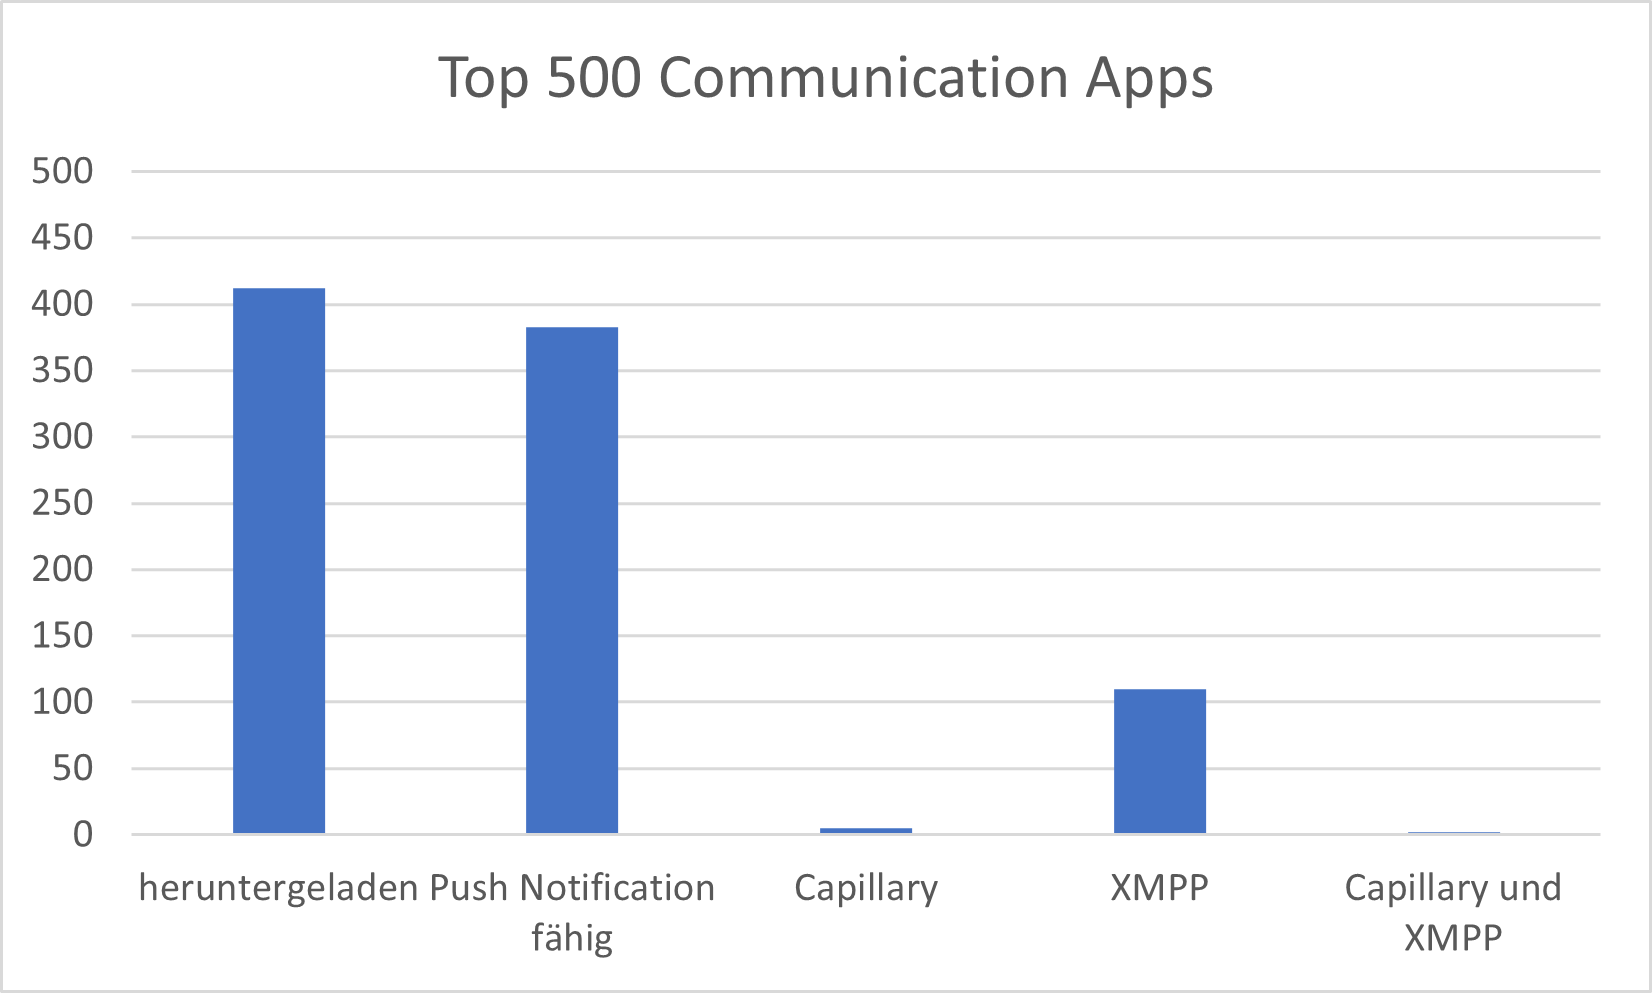
\includegraphics[width=\linewidth]{sample-auswertung1}
  \caption{Top 500 Communication Apps.}
  \Description{Graph Auswertung der Top 500 Communication Apps}
\end{figure}
Von 500 Apps wurden 413 heruntergeladen, 393 benutzen "NotificationCompat" oder "onMessageReceived" 
und sind somit in der Lage Push Notification abzuschicken sowie von Firebase zu empfangen. Davon benutzen 5 Apps Capillary, 115 Apps XMPP 
und 2 Apps benutzen beides.

\subsection{Top 500 Health and Fitness Apps}
\begin{figure}[H]
  \centering
  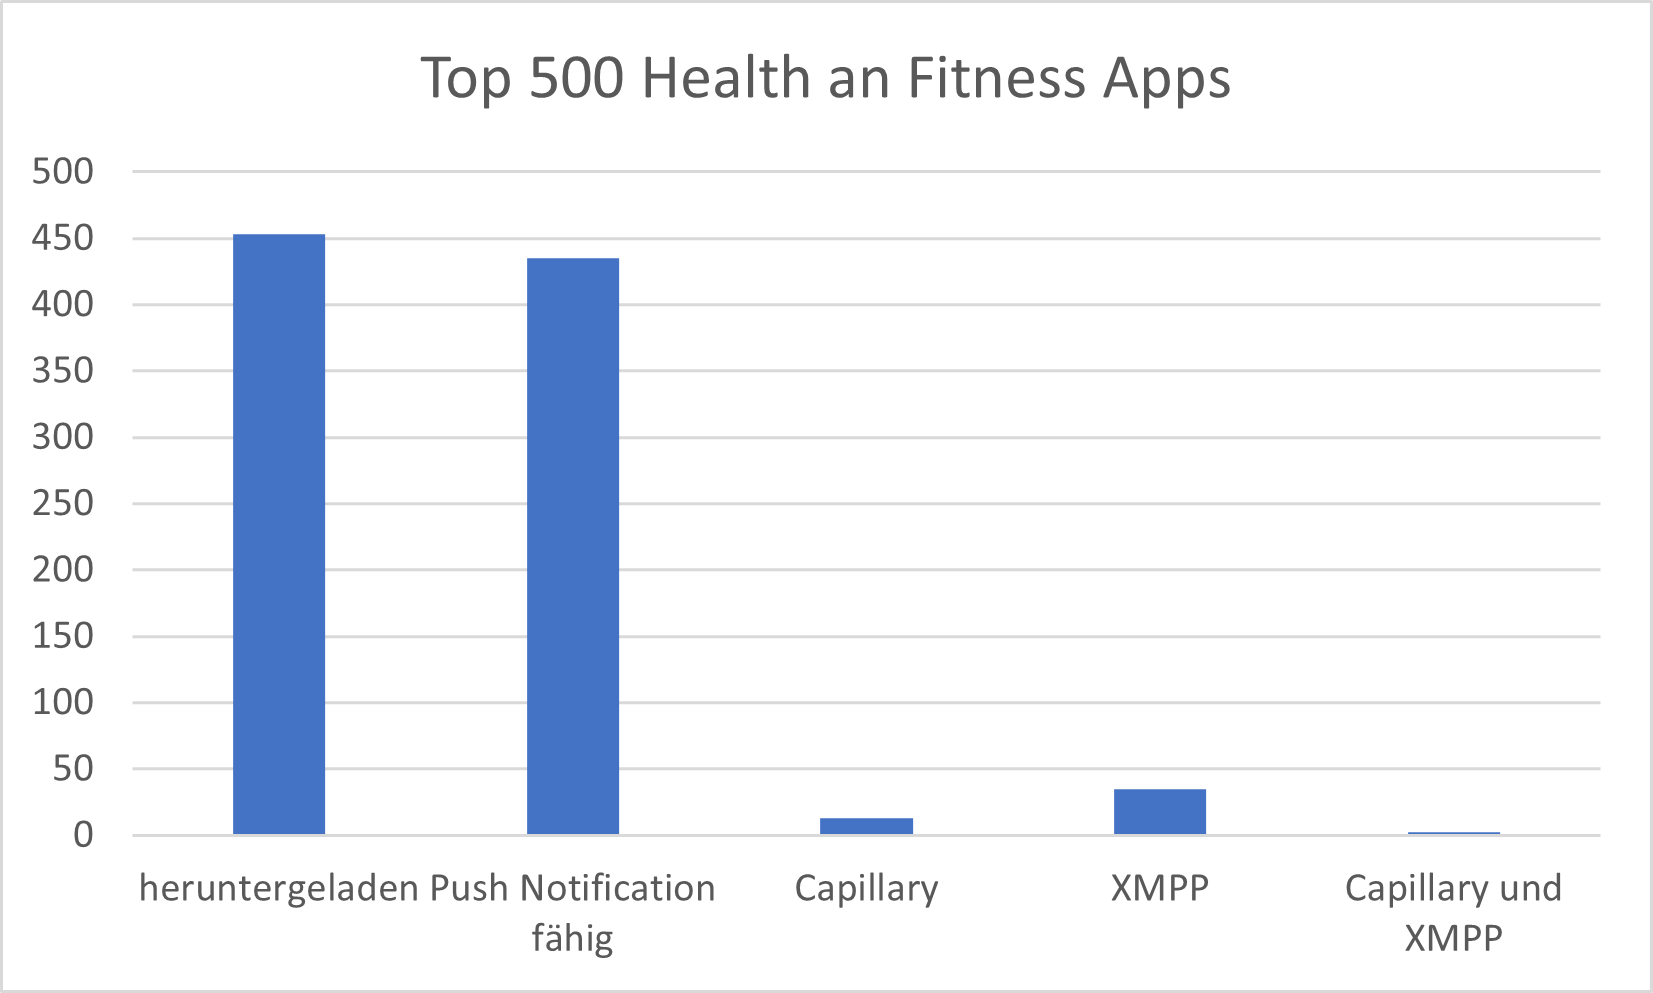
\includegraphics[width=\linewidth]{sample-auswertung2}
  \caption{Top 500 Health and Fitness Apps.}
  \Description{Graph Auswertung der Top 500 Health and Fitness Apps}
\end{figure}
Von 500 Apps wurden 453 heruntergeladen, 435 benutzen "NotificationCompat" oder "onMessageReceived" 
und sind somit in der Lage Push Notification abzuschicken sowie von Firebase zu empfangen. Davon benutzen 13 Apps Capillary, 
35 Apps XMPP und 2 Apps benutzen beides.

\subsection{Top 500 Medical Apps}

\begin{figure}[H]
  \centering
  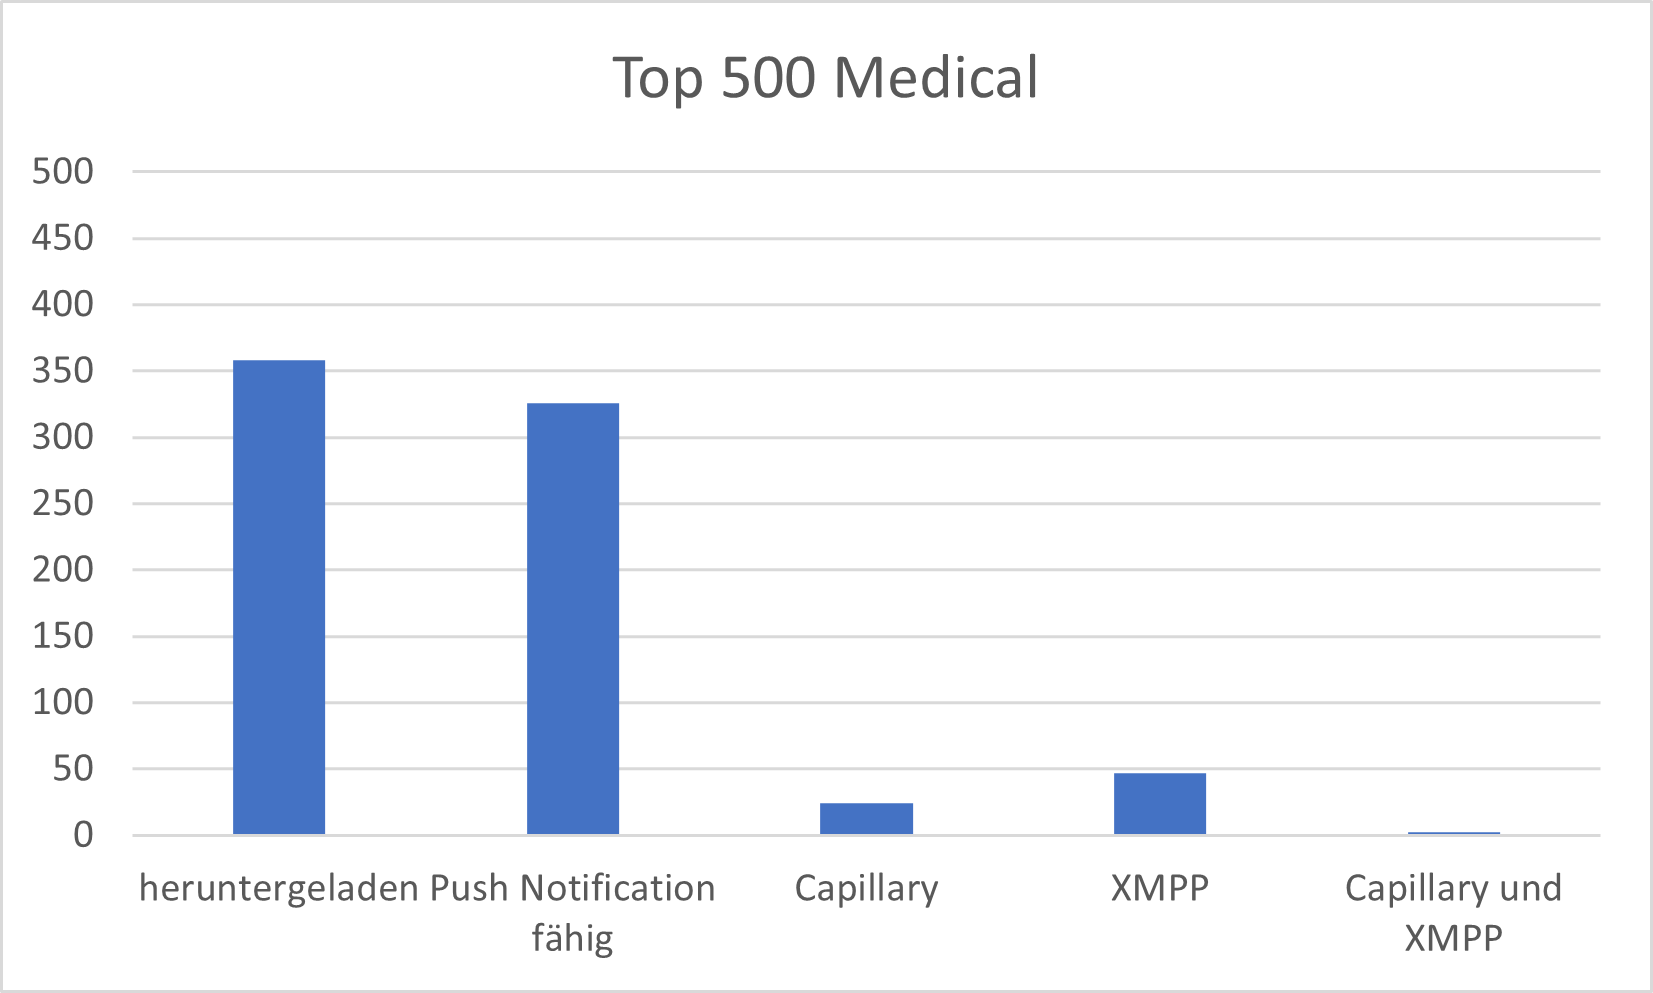
\includegraphics[width=\linewidth]{sample-auswertung3}
  \caption{Top 500 Medical Apps.}
  \Description{Graph Auswertung der Top 500 Medical Apps}
\end{figure}

Von 500 Apps wurden 358 heruntergeladen, 326 benutzen "NotificationCompat" oder "onMessageReceived" 
und sind somit in der Lage Push Notification abzuschicken sowie von Firebase zu empfangen. Davon benutzen 24 Apps Capillary, 
47 Apps XMPP und 2 Apps benutzen beides.

\subsection{Auswertung}
Es fällt auf, dass Capillary im medizinischen Bereich mit 24 Apps am meisten vor kommt, während XMPP im Bereich
der Kommunikation mit 110 Apps am meisten vor kommt. Generell sind die Zahlen niedrig.
 Allerdings sind die Zahlen mit Vorsicht zu genießen, da die
Analyse nicht auf obfsukierte Apps angepasst wurde, zudem wurde nicht überprüft, ob die Apps mit XMPP auch verschlüsselte 
Push Notifications unterstützen und zuletzt können manche der Apps eigene End-to-End Push Notification Lösungen benutzen.

\subsection{Ausbaufähigkeit}
Unser Skript lässt sich theoretisch erweitern um einen robusteren Download. Der Download könnte mit mit 
mehreren Google Accounts und zusätzlich über Proxy Server realisiert werden, um eine Drosselung von Google 
zu minimieren.
Die Analysemethodik kann weiterhin ausgebaut werden, indem Lösungen für die oben genannten Probleme gefunden werden.
Eine mögliche Lösung wäre einen Smali Parser zu entwickeln, der Zusammenhänge zwischen Android Schnittstellen ausfindig macht
und somit eine mögliche Verschlüsselung von Push Notification anzeigen kann. Eine weitere mögliche Lösung könnte durch SSL Interception
realisiert werden, indem der Verkehr zwischen der App und dem Push Notification Cloud Service analysiert wird.

%%
%% The next two lines define the bibliography style to be used, and
%% the bibliography file.
\bibliographystyle{ACM-Reference-Format}
\bibliography{sample-base}


\end{document}
\endinput
%%
%% End of file `sample-sigconf.tex'.
